\documentclass[a4paper,10pt]{report}
\usepackage{fancyhdr} % heading & footer
\usepackage[spanish,activeacute]{babel}
\usepackage{amssymb}
\usepackage{amsmath}
\pagestyle{fancy}
\usepackage{alltt}
% with this we ensure that the chapter and section
% headings are in lowercase.
\renewcommand{\chaptermark}[1]{%
        \markboth{#1}{}}
\renewcommand{\sectionmark}[1]{%
        \markright{Sec \thesection\ - #1}}
\fancyhf{} % delete current header and footer
\fancyhead[LE,RO]{\textit\thepage}
\fancyhead[LO]{\bfseries\textit\rightmark}
\fancyhead[RE]{\bfseries\textit\leftmark}
\renewcommand{\headrulewidth}{0.5pt} % width linea
\renewcommand{\footrulewidth}{0pt}
\addtolength{\headheight}{13pt} % space for the rule
\fancypagestyle{plain}{%
   \fancyhead{} % get rid of headers on plain pages
   \renewcommand{\headrulewidth}{0pt} % and the line
}

\usepackage{graphicx}
\usepackage{listings}
\usepackage{xcolor}
\usepackage{multirow}
\usepackage[l3]{csvsimple}
\renewcommand{\lstlistingname}{Código}
\usepackage{tikz}
\usetikzlibrary{shapes, arrows, positioning}

\usepackage[all]{xy}

\usepackage{listings}

\usepackage{setspace}

\usepackage{epigraph}
\usepackage{etoolbox}
\setlength\epigraphwidth{8cm}
\setlength\epigraphrule{0pt}
\makeatletter
\patchcmd{\epigraph}{\@epitext{#1}}{\itshape\@epitext{#1}}{}{}
\makeatother

\usepackage{color}
\usepackage{textcomp}
\definecolor{listinggray}{gray}{0.9}
\definecolor{lbcolor}{rgb}{0.95,0.95,0.95}

%
%
%
\usepackage{array}
\usepackage{xr}
\usepackage[utf8]{inputenc}



% Algunos parametros para los margenes
\oddsidemargin 0in \headsep 0.5cm
\textwidth=16.54cm \textheight=22cm
\headwidth=16.54cm

% Configuración del estilo para el lenguaje Bash
\lstdefinestyle{bashstyle}{
    language=bash,
    basicstyle=\ttfamily\small,       % Fuente y tamaño
    commentstyle=\color{gray},       % Estilo de los comentarios
    keywordstyle=\color{black}\bfseries,       % Estilo de las palabras clave
    stringstyle=\color{black}\bfseries, % Estilo de las cadenas de texto (negrita en negro)    showstringspaces=false,          % No mostrar espacios en cadenas de texto
    breaklines=true,                 % Romper líneas largas automáticamente
    breakatwhitespace=true,          % Romper solo en espacios en blanco
    numbers=left,                    % Números de línea a la izquierda
    numberstyle=\tiny\color{gray},   % Estilo de los números de línea
    frame=single,                    % Borde alrededor del código
    captionpos=b,                    % Posición de la leyenda (abajo)
    xleftmargin=25pt,                % Margen izquierdo
    xrightmargin=15pt,               % Margen derecho
    framexleftmargin=20pt,           % Margen izquierdo dentro del borde
    framexrightmargin=20pt,           % Margen izquierdo dentro del borde
    framextopmargin=5pt,             % Margen superior dentro del borde
    framexbottommargin=5pt,          % Margen inferior dentro del borde
}

% Configuración del estilo para el lenguaje Java
\lstdefinestyle{javastyle}{
    language=Java,
    basicstyle=\ttfamily\small,       % Fuente y tamaño
    commentstyle=\color{gray},       % Estilo de los comentarios
    keywordstyle=\color{black}\bfseries,       % Estilo de las palabras clave
    stringstyle=\color{black}\bfseries, % Estilo de las cadenas de texto (negrita en negro)
    showstringspaces=false,          % No mostrar espacios en cadenas de texto
    breaklines=true,                 % Romper líneas largas automáticamente
    breakatwhitespace=true,          % Romper solo en espacios en blanco
    numbers=left,                    % Números de línea a la izquierda
    numberstyle=\tiny\color{gray},   % Estilo de los números de línea
    frame=single,                    % Borde alrededor del código
    captionpos=b,                    % Posición de la leyenda (abajo)
    xleftmargin=25pt,                % Margen izquierdo
    xrightmargin=15pt,               % Margen derecho
    framexleftmargin=20pt,           % Margen izquierdo dentro del borde
    framextopmargin=5pt,             % Margen superior dentro del borde
    framexbottommargin=5pt,          % Margen inferior dentro del borde
}

\title{
\Huge {Aserciones de tests vs contratos en el testing de regresión: Un estudio de efectividad}\\
}

\date{\vspace*{1\baselineskip}---\\ Departamento de Computación \\
      Facultad de Cs. Exactas Físico-Químicas y Naturales \\
      Universidad Nacional de R\'io Cuarto\\ 
	  \vspace*{1\baselineskip}      
      ---\\
      \vspace*{1\baselineskip} 
      {\bf Director:} Dr. Facundo Molina\\
      {\bf Codirector:} Dr. Nazareno Aguirre\\
      \vspace*{2\baselineskip}
      \today
      }

\LARGE{\author{Claudio Dosantos}}

\begin{document}
\setcounter{chapter}{0}
\maketitle

\newpage

\chapter{Introducción}

% Plantear marco general
% En esta sección, se presenta una introducción al problema del oráculo, los diferentes tipos de oráculos y cómo se mide la calidad de los mismos.

La calidad de los sistemas de software típicamente se define alrededor de varios aspectos, tales como confiabilidad, usabilidad, eficiencia, etc. Entre ellos, la confiabilidad es generalmente considerada una característica fundamental en lo que respecta a la calidad del software, y de gran interés en el proceso de desarrollo de software [0]. 

Analizar la calidad del software está fuertemente relacionado con la tarea de encontrar defectos en el mismo, es decir, identificar algún comportamiento actual del software que difiera del comportamiento esperado. En este sentido, si se considera un determinado dato de entrada para un sistema, el desafío de distinguir el comportamiento correcto de uno incorrecto es conocido como el problema del oraculo []. Es esperable que esta tarea se pueda realizar con el menor costo posible y con los mayores beneficios, garantizando que el sistema funcione correctamente para distintos valores de entrada. 
Se han introducido técnicas para oráculos automáticos como modelado, especificaciones, desarrollo guiado por contratos, y testing metamorfico. Aún así existen casos donde ninguna de estas técnicas son adecuadas, por lo que la intervención manual del desarrollador es necesaria.

Las especificaciones de software pueden aparecer de diversas maneras. A nivel de código fuente, cuando están presentes, generalmente se manifiestan o bien como comentarios, es decir, descripciones informales en lenguaje natural de lo que se supone que debe hacer el software, o más formalmente como aserciones de programas, es decir, declaraciones (normalmente ejecutables) que capturan propiedades que el software debe satisfacer en ciertos puntos durante su ejecución. Las especificaciones como comentarios son más comunes, pero tiene la desventaja de que no pueden utilizarse de manera directa para el análisis automático de confiabilidad. 
Deido a esta situación, el problema de inferencia de especificaciones (un caso especial del conocido problema del oráculo [Barr et al. 2015]), es decir, el problema de generar una descripción formal del comportamiento del software a partir de elementos existentes (documentación, código fuente, etc.), ha recibido una atención cada vez mayor por parte de la comunidad de Ingeniería de Software.

En las últimas décadas, con el objetivo de ayudar a los desarrolladores a equipar las implementaciones con especificaciones, se han desarrollado una variedad de técnicas de inferencia automática de aserciones de regresión, es decir, aserciones que capturan el comportamiento actual del software. Estas técnicas, generalmente basadas en observaciones de ejecuciones del software bajo análisis, pueden producir distintos tipos de aserciones de regresión. Por ejemplo, algunas técnicas de generación automática de tests [Fraser & Arcuri 2011, Pacheco & Ernst 2007] incorporan mecanismos para producir aserciones de test, es decir, aserciones que capturan propiedades válidas en un escenario (test) específico. Por otro lado, otras técnicas de inferencia de especificaciones [Ernst et al. 2007, Le & Lo 2018, Molina et al. 2019, Molina et al. 2021, Molina et al. 2022, Terragni et al. 2020] son capaces de inferir aserciones de contratos, es decir, aserciones más generales asociadas con elementos de contratos como precondiciones, postcondiciones e invariantes [Meyer 1992].

\section{Problema}

La principal hipótesis de trabajo es que el tipo de aserciones de regresión utilizadas en testing de regresión, ya sean aserciones de test o aserciones de contratos, puede tener un impacto considerable en la efectividad del análisis para detectar defectos producidos por cambios en el software.

El objetivo principal de este trabajo es el estudio y análisis de la efectividad de distintas aserciones de regresión para detectar errores durante la tarea de testing de regresión. Esencialmente, se desea analizar la efectividad de las aserciones de test en comparación con las aserciones de contratos. Para esta tarea, se propone, para diversos casos de estudio de la literatura, simular escenarios de testing de regresión utilizando, por un lado, aserciones de test, y por otro, aserciones de contratos, generadas automáticamente.

En particular se pone el foco en las aserciones generadas por herramientas del estado del arte de generación automática de tests como Randoop[0] y Daikon[0]. 

A modo de ejemplo consideremos la implementación de nodo de listas doblemente enlazadas con su método insertRight.

\begin{figure}[ht]
\centering
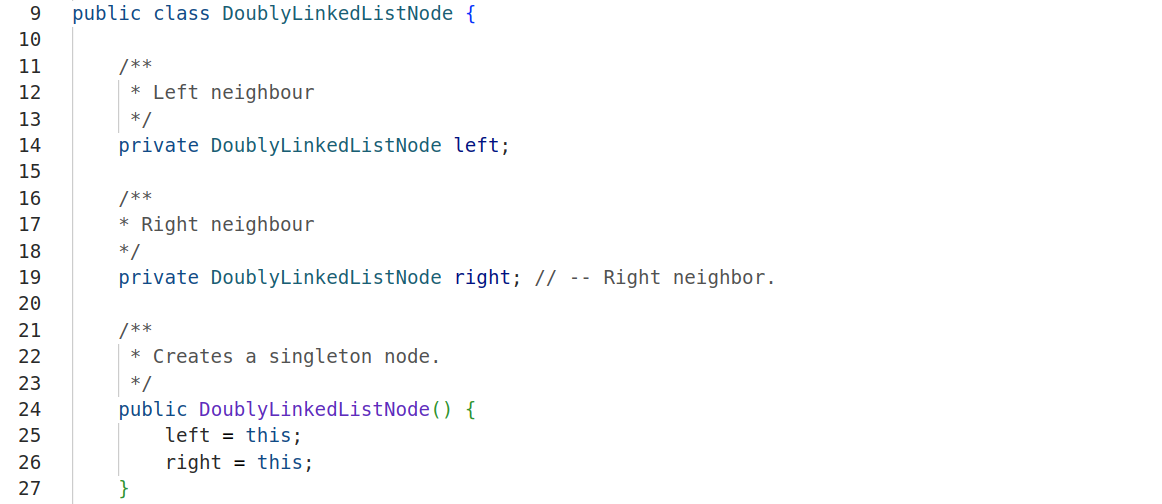
\includegraphics[width=1\textwidth]{doublelinkedlistnode/constructor.png}
\caption{DoubleLinkedListNode}
\label{fig:DoubleLinkedListNode}
\end{figure}


\begin{figure}[ht]
\centering
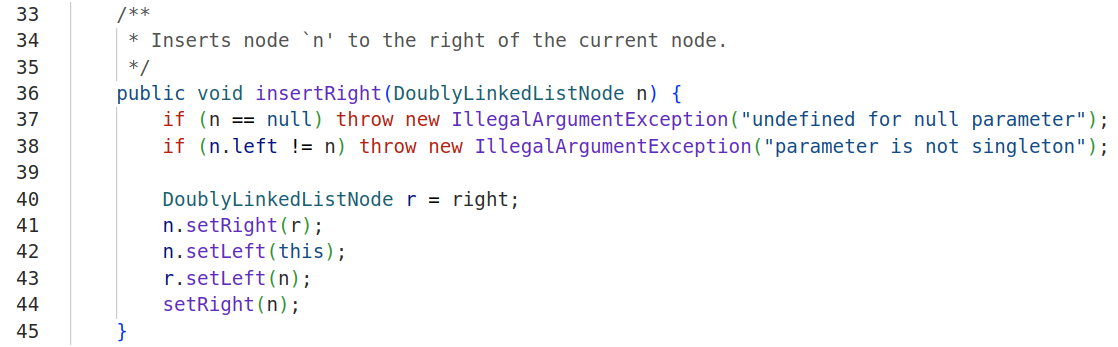
\includegraphics[width=1\textwidth]{doublelinkedlistnode/insertRight.png}
\caption{DoubleLinkedListNode.insertRight}
\label{fig:DoubleLinkedListNodeInsertRight}
\end{figure}

A modo de ilustración en la siguiente imágen se puede ver un caso de test generado por Randoop y un contrato generado por Daikon.

\begin{figure}[ht]
\centering
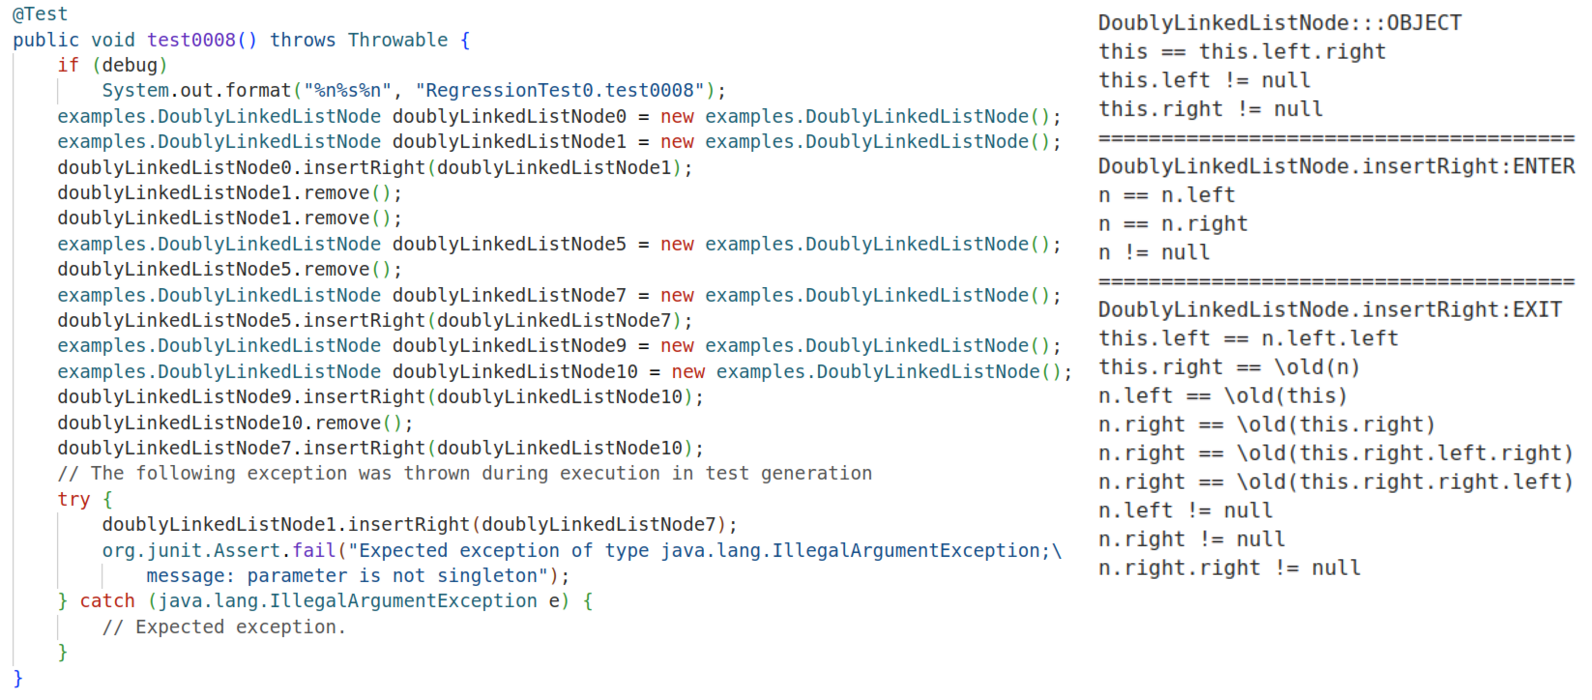
\includegraphics[width=1\textwidth]{doublelinkedlistnode/randoop-daikon-example.png}
\caption{Test y contrato generados automáticamente por Randoop y Daikon respectivamente para el método insertRight}
\label{fig:DoubleLinkedListNodeTests}
\end{figure}

\chapter{Generación Automática de Oráculos}

La generación automática de oráculos es una técnica innovadora en el campo de la verificación y validación de software que busca abordar uno de los desafíos más complejos en el proceso de pruebas: la creación confiable y precisa de oráculos de prueba.

En el contexto de las pruebas de software, un oráculo es un mecanismo que compara los resultados esperados de un programa con los resultados reales obtenidos durante la ejecución de las pruebas. El oráculo determina si el programa se comporta correctamente o si existen discrepancias que indiquen la presencia de errores o fallos.

La generación automática de oráculos tiene como objetivo reducir la intervención manual en la creación de estos oráculos, lo que a menudo es una tarea laboriosa y propensa a errores. Utilizando un conjunto diverso de técnicas que incluyen inteligencia artificial, machine learning, análisis estático, dinámico y también técnicas aleatorias, esta metodología permite inferir o construir automáticamente oráculos precisos y efectivos para diferentes tipos de pruebas.

\section{Unit Assertions con Randoop/EvoSuite}

\subsection{Randoop}

Randoop propone una mejora a la generación de pruebas aleatorias mediante la utilización de una técnica llamada generación de pruebas aleatorias dirigidas por retroalimentación (Feedback-directed Random Test Generation).

El enfoque de Randoop se basa en generar secuencias de invocaciones a métodos de las clases bajo prueba de forma aleatoria. Estas secuencias, que se crean inicialmente, luego se combinan para obtener nuevas secuencias. A continuación, se someten a una serie de evaluaciones mediante contratos y filtros, como la detección de excepciones, errores de aserciones o incluso la comparación con secuencias previamente generadas. Las secuencias que superan estas validaciones son seleccionadas como candidatas prometedoras para generar nuevas secuencias y, posteriormente, se pueden utilizar como tests de regresión para asegurar la calidad y funcionalidad continua del sistema bajo prueba.

Por otro lado, las secuencias que no cumplen con uno o más de los contratos establecidos indican la presencia potencial de errores en el sistema bajo prueba. Estas secuencias problemáticas se convierten en valiosos hallazgos para los equipos de desarrollo, ya que apuntan a áreas críticas que requieren correcciones y mejoras.

El enfoque de generación de pruebas aleatorias dirigidas por retroalimentación de Randoop representa un intento significativo para mejorar la efectividad del testing aleatorio al combinarlo con criterios de selección más inteligentes y evaluaciones de calidad. Al hacerlo, se logra una mayor cobertura de pruebas y se descubren más escenarios de prueba, lo que puede llevar a una mejor detección y corrección de errores en el software bajo evaluación. Este enfoque se ha mostrado prometedor en muchos entornos de desarrollo y se considera una herramienta valiosa para la mejora del proceso de testing en el desarrollo de software.


\subsection{EvoSuite}

EvoSuite es una herramienta de generación automática de conjuntos de pruebas para software orientado a objetos, que emplea un enfoque basado en algoritmos de búsqueda. Esta técnica combina diversas estrategias, como búsqueda híbrida, ejecución simbólica dinámica y transformación de testabilidad, para lograr una generación de pruebas más eficiente y efectiva.

Uno de los aspectos clave de EvoSuite es la utilización de algoritmos genéticos en su proceso de generación de pruebas. Estos algoritmos genéticos se inspiran en la evolución biológica y aplican operadores genéticos como selección, cruce y mutación en poblaciones de pruebas para mejorar la cobertura y calidad de los casos de prueba generados.

EvoSuite emplea dos técnicas principales:

1. Generación del conjunto de pruebas completo (Whole test suite generation):
En lugar de optimizar metas de cobertura individuales, EvoSuite se enfoca en optimizar un criterio de cobertura general. Esto evita que el resultado se vea negativamente influenciado por el orden o la dificultad de alcanzar metas de cobertura individuales. Al optimizar la cobertura de manera integral, la herramienta puede producir conjuntos de pruebas más completos y representativos.

2. Generación de aserciones basada en mutaciones (Mutation-based assertion generation):
Esta técnica se centra en evaluar la efectividad de los casos de prueba generados. Para ello, se ejecutan las pruebas en unidades de prueba (UUT) con algunas modificaciones o mutaciones en el código. Aquellas pruebas que detecten los errores introducidos por las mutaciones reciben una mejor puntuación, ya que se consideran más valiosas. Finalmente, se selecciona el subconjunto más pequeño de pruebas que es capaz de detectar las mutaciones, lo que garantiza una cobertura efectiva y eficiente de las posibles fallas en el software.

La combinación de búsqueda híbrida, ejecución simbólica dinámica y transformación de testabilidad, junto con el uso de algoritmos genéticos, hacen que EvoSuite sea una herramienta poderosa para la generación automática de conjuntos de pruebas. Esta aproximación ha demostrado ser efectiva en diversos contextos de desarrollo de software, y ha ayudado a mejorar la calidad y confiabilidad de los programas bajo prueba.


\section{Contratos con Daikon}

Daikon es una herramienta que emplea técnicas de aprendizaje automático para llevar a cabo la detección dinámica de posibles invariantes en el código de programas. Utiliza datos recopilados durante múltiples ejecuciones del programa para analizar patrones y descubrir propiedades que se mantienen constantes a lo largo de todas las ejecuciones.

A través de un proceso de aprendizaje automático, Daikon busca identificar invariantes relevantes que puedan ser representativos del comportamiento general del programa. Estas propiedades se consideran como reglas generales que deben cumplirse en todas las instancias del programa.

Daikon utiliza una gramática de propiedades y variables para definir qué tipo de invariantes buscar. Las propiedades pueden ser de diferentes formas, como comparaciones numéricas, relaciones entre variables, o incluso estructuras de datos complejas. Las variables representan los valores que se recopilan durante la ejecución del programa.

Las aplicaciones de Daikon son diversas y abarcan desde la documentación del programa, hasta la detección y prevención de errores (bugs), debugging, testing, verificación de propiedades, análisis de estructuras de datos y corrección de inconsistencias.


\section{Contratos con SpecFuzzer}

SpecFuzzer es una técnica que se utiliza para...

\section{Ejemplos de generación de oráculos}

\begin{lstlisting}[style=javastyle, caption=Ejemplo StackAr.top, label=lst:top]
/**
 * Array-based implementation of the stack.
 * @author Mark Allen Weiss
 */
public class StackAr {
    /**
     * Construct the stack.
     * @param capacity the capacity.
     */
    public StackAr( int capacity )
    {
        theArray = new Object[ capacity ];
        topOfStack = -1;
    }

    /**
     * Test if the stack is logically empty.
     * @return true if empty, false otherwise.
     * @observer // annotation added by Jeremy
     */
    public boolean isEmpty( )
    {
        return topOfStack == -1;
    }

    /**
     * Get the most recently inserted item in the stack.
     * Does not alter the stack.
     * @return the most recently inserted item in the stack, or null, if empty.
     * @observer // annotation added by Jeremy
     */
    public Object top( )
    {
        if( isEmpty( ) )
            return null;
        Object result = theArray[ topOfStack ];
    	assert(true);
        return result;
    }
}
\end{lstlisting}


\subsection{Randoop}.


\begin{lstlisting}[style=javastyle, caption=Aserción generada con Randoop, label=lst:randoop]
@Test
public void test062() throws Throwable {
    if (debug)
        System.out.format("%n%s%n", "RegressionTest0.test062");
    DataStructures.StackAr stackAr1 = new DataStructures.StackAr(6);
    boolean boolean2 = stackAr1.isEmpty();
    stackAr1.push((java.lang.Object) 5L);
    boolean boolean5 = stackAr1.isEmpty();
    stackAr1.pop();
    java.lang.Object obj7 = stackAr1.top();
    stackAr1.makeEmpty();
    org.junit.Assert.assertTrue("'" + boolean2 + "' != '" + true + "'", boolean2 == true);
    org.junit.Assert.assertTrue("'" + boolean5 + "' != '" + false + "'", boolean5 == false);
    org.junit.Assert.assertNull(obj7);
}
\end{lstlisting}


\subsection{Daikon}

\begin{lstlisting}[style=javastyle, caption=Aserción generada con Daikon, label=lst:daikon]
DataStructures.StackAr.top():::EXIT76
daikon.Quant.eltsEqual(this.theArray, null)
daikon.Quant.eltsEqual(daikon.Quant.typeArray(this.theArray), null)
this.topOfStack == -1
\result == null
daikon.Quant.eltsEqual(this.theArray, \result)

\end{lstlisting}
\chapter{Mutation Testing}

El concepto de Pruebas de Mutación (Mutation Testing) se introdujo en la década de 1970 como un método para evaluar la efectividad de un conjunto de pruebas en la detección de fallas y para identificar sus puntos débiles.

El enfoque de las Pruebas de Mutación implica la inserción deliberada de defectos comunes en el código fuente, creando así versiones modificadas del programa llamadas mutantes. Luego, estos mutantes se someten a la ejecución del conjunto de pruebas existente, con el propósito de verificar si los defectos son detectados por las pruebas o no.

Un mutante que es detectado y produce un fallo se considera "muerto" y se descarta como no relevante. Por el contrario, aquellos mutantes que no son detectados (llamados "vivos") revelan posibles debilidades en el conjunto de pruebas, ya que representan fallas potenciales no detectadas.

La calidad de un conjunto de pruebas se evalúa según la cantidad de mutantes detectados. Si un conjunto de pruebas no logra detectar mutantes, se considera débil y propenso a contener fallas no detectadas. Por el contrario, cuantos más mutantes sean detectados por las pruebas, mayor será la confiabilidad del conjunto de pruebas y la capacidad para encontrar posibles errores.

Por todas estas razones, utilizar Mutation Testing para evaluar la calidad de las pruebas y los invariantes generados es un enfoque confiable y efectivo. Al someter el software a mutantes deliberados y analizar cómo las pruebas responden ante estas versiones modificadas, se puede obtener una evaluación objetiva de la capacidad de detección de fallas del conjunto de pruebas y, en consecuencia, identificar áreas de mejora en el proceso de pruebas y desarrollo de software.


\section{Major}

Major es un framework usado para el análisis de mutación en el ámbito de la programación y prueba de software.

\subsection{Operadores de mutación}

Major incluye los siguientes operadores de mutación: 

\begin{itemize}
  \item AOR (Arithmetic Operator Replacement), el cual reemplaza operadores aritméticos binarios por otros compatibles. Ej: a + b ==> a - b
  \item COR (Conditional Operator Replacement), el cual reemplaza operadores condicionales por otros compatibles. Ej: a || b ==> a && b
  \item LOR (Logical Operator Replacement), el cual reemplaza operadores lógicos por otros compatibles. Ej: a ^ b ==> a | b
  \item ROR (Relational Operator Replacement), el cual reemplaza operadores relacionales por otros compatibles. Ej: a == b ==> a >= b
  \item SOR (Shift Operator Replacement), el cual reemplaza operadores de desplazamientos de bits por otros compatibles. Ej: a >> b ==> a << b
  \item ORU (Operator Replacement Unary), el cual reemplaza operadores unarios por otros compatibles. Ej: -a ==> ~a
  \item LVR (Literal Value Replacement), el cual reemplaza un literal por un valor por defecto. Ej: val = 0 ==> 1 and -1
  \item EVR (Expression Value Replacement), el cual reemplaza una expresión por un valor por defecto. Ej: return a ==> return 0
  \item STD (Statement Deletion), Omite sentencias simples del tipo return, break, continue, llamadas a métodos, asignaciones, pre y pos incremento.
\end{itemize}


\subsection{Para el ejemplo de la sección 2}

\begin{lstlisting}[style=javastyle, caption=Mutaciones StackAr.top, label=lst:major]
31:COR:isEmpty():TRUE:DataStructures.StackAr@top():75:isEmpty() |==> false
32:COR:isEmpty():FALSE:DataStructures.StackAr@top():75:isEmpty() |==> true
33:STD:<RETURN>:<NO-OP>:DataStructures.StackAr@top():76:return null; |==> <NO-OP>
34:EVR:<ARRAY_ACCESS(java.lang.Object)>:<DEFAULT>:DataStructures.StackAr@top():77:theArray[topOfStack] |==> null
35:LVR:TRUE:FALSE:DataStructures.StackAr@top():78:true |==> false
36:EVR:<IDENTIFIER(java.lang.Object)>:<DEFAULT>:DataStructures.StackAr@top():79:result |==> null
\end{lstlisting}

\chapter{Análisis de Efectividad de los Oráculos}

En esta sección, se presenta el diseño del experimento realizado para evaluar la efectividad de los oráculos generados automáticamente. También se presentan los resultados obtenidos.

\section{Evaluación Experimental}

Se describe el diseño del experimento y cómo se evaluaron los oráculos generados.

\subsection{Generación de oráculos}

Para comparar la eficiencia de pruebas de regresión generadas con distintos enfoques, aserciones de test y contratos se plantean los siguientes pasos. 

Dado un código que representa una solución correcta a un problema específico, como primer paso se deben generar casos de pruebas utilizando las herramientas de generación automática mencionadas en el Capítulo 2.

1) Generación de tests utilizando Randoop.
A partir del archivo ejecutable del código bajo prueba, la clase y el método a probar. Obtendremos aserciones como hemos visto en el Código 2.2 de la sección 2.4.1.


\begin{lstlisting}[style=bashstyle, caption=Generación de tests con Randoop, label=lst:bashcode]
java -cp ${randoop_jar}:${project_classpath} randoop.main.Main gentests $test_classes --classlist=$classlist --serialize-folder=$mutator_inputs --serialize-method=\"$regex_method\" --junit-package-name=$package --junit-output-dir=$outdir_tests --junit-reflection-allowed=false --time-limit=$timelimit --literals-level=ALL --literals-file=$literals --omit-methods=\"$omitmethods\"
\end{lstlisting}


2) Generación de aserciones utilizando Daikon. 
A partir de los archivos ejecutables de las pruebas generadas con Randoop, el código bajo prueba, el nombre de la clase y el método a probar, al ejecutar el siguiente script se obtienen aserciones Daikon como se ha visto en el Código 2.3 de la sección 2.4.2.

\begin{lstlisting}[style=bashstyle, caption=Generación de tests con Randoop, label=lst:bashcode]
# First step: perform dynamic comparability analysis (with DynComp)
java -cp \
 ${tests_bin}:${daikon_path}/daikon.jar:${subject_jar} \
 daikon.DynComp --output-dir=${output_dir}daikon/ \
 ${package}.RegressionTestDriver

# Second step: obtain the dtrace file with Chicory
echo '--> Going to run Chicory'
java -cp \
 ${tests_bin}:${daikon_path}/daikon.jar:${subject_jar} \
 daikon.Chicory --comparability-file=\
 ${output_dir}daikon/RegressionTestDriver.decls-DynComp \
 --output-dir=${output_dir}daikon/ ${package}.RegressionTestDriver

# Third step: actual Daikon execution to infer specs
echo '--> Going to run Daikon'
java -cp ${daikon_path}/daikon.jar daikon.Daikon \
 --ppt-select-pattern \
 ${package}'\.'$2':::CLASS|'${package}'\.'$2':::OBJECT|\
 '${package}'\.'$2'\.'$method_without_args \
 -o ${output_dir}daikon/res.inv.gz \
 ${output_dir}daikon/RegressionTestDriver.dtrace.gz

# Process result and print the Daikon specs for better readability. First
# the ones related to class invariants, and then the ones related to the current method
java -cp ${daikon_path}/daikon.jar daikon.PrintInvariants \
 ${output_dir}daikon/res.inv.gz --format java > ${output_dir}daikon/res.txt
\end{lstlisting}


3) Generación y compilación de mutantes utilizando Major.

\begin{lstlisting}[style=bashstyle, caption=Generación de mutantes con Major, label=lst:bashcode]
$major/bin/javac -cp $subject_jar -nowarn -J-Dmajor.export.mutants=true -XMutator:ALL \
 -d ${output_dir}bin ${source_dir}src/main/java/$class_path/${2}.java
\end{lstlisting}


4) Ejecución de las aserciones generadas por Randoop sobre cada mutante.
Para cada ejecución se analiza la salida, básicamente puede obtenerse como resultado que las aserciones no encuentran errores o por el contrario si lo encuentran, es decir que detectan la mutación. En este último caso, a su vez es necesario identificar aquellas ejecuciones en las que las aserciones fallan, de las que son ejecuciones erroneas.
En la siguiente tabla se puede visualizar un ejemplo del resultado obtenido.

\vspace{10pt}

\csvautotabular{stackAr-top-randoop-result.csv}

\vspace{10pt}

5) Ejecución de las aserciones generadas por Daikon sobre cada mutante. En la siguiente tabla se pueden ver los resultados obtenidos para el ejemplo.

\vspace{10pt}

\csvautotabular{stackAr-top-daikon-result.csv}

\vspace{10pt}


\section{Resultados}

Se presentan los resultados obtenidos en el experimento y se analizan.

\begin{figure}[ht]
\centering
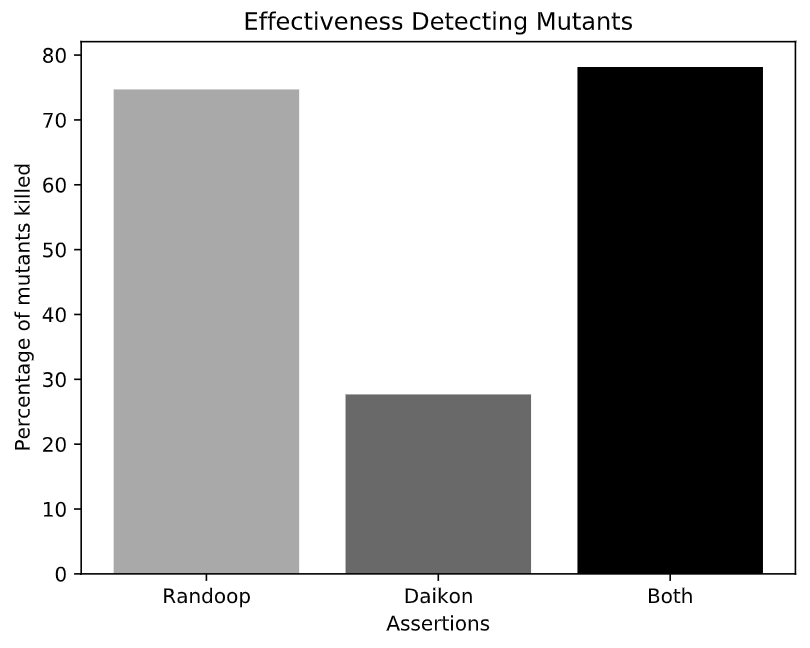
\includegraphics[width=0.8\textwidth]{tools-effectiveness.png}
\caption{Resultados obtenidos}
\label{fig:nombre_etiqueta}
\end{figure}

\vspace{10pt}

\csvautotabular{effectiveness.csv}

\vspace{10pt}



Graficos y Tablas segun mutante

\vspace{10pt}

\csvautotabular{effectiveness-by-mutant-type.csv}

\vspace{10pt}
\chapter{Conclusiones}

En esta sección, se presentan las principales conclusiones basadas en los resultados obtenidos en el experimento. También se mencionan posibles direcciones para trabajo futuro.



\end{document}
